\documentclass[12pt, singlespace]{article}
\usepackage{graphicx} %graphics
\usepackage{float} % for use [H] - force tables and image to place where you want
\usepackage[utf8]{inputenc}
\usepackage{amsmath}
\usepackage{amssymb}
\let\proof\relax 
\let\endproof\relax 
\usepackage{amsthm}
\usepackage{times}
\usepackage{url}
\usepackage{xspace}
\usepackage{comment}
\usepackage{color}
\usepackage{thmtools, thm-restate}
\usepackage{algorithm}
\usepackage[noend]{algorithmic}
\usepackage{booktabs}
\usepackage{tabulary}
\usepackage[margin=1in]{geometry}
\usepackage{multirow}
\usepackage{breakcites} % break citations that overflow lines
\usepackage{verbatim} % for comment
\usepackage{cite}
\usepackage{subfigure}

\renewcommand{\figurename}{Figure}
\newcommand{\cnote}[1]{\footnote{\textcolor{black}{#1}}}


\pagestyle{plain} % shows page number

\title{ 597I Data Privacy Final Report}
\author{Chen Sun$^{\dagger}$}




% this block of code replaces the letter l by \ell in math mode
\mathcode`l="8000
\begingroup
\makeatletter
\lccode`\~=`\l
\DeclareMathSymbol{\lsb@l}{\mathalpha}{letters}{`l}
\lowercase{\gdef~{\ifnum\the\mathgroup=\m@ne \ell \else \lsb@l \fi}}%
\endgroup

%\setlength{\parskip}{0pt} % trick to save some space

\begin{document}

\maketitle
\let\thefootnote\relax\footnotetext{$^\dagger$Corresponding author, chensun@cse.psu.edu}
\section{Introduction}
\subsection{Background}

From the perspective of computer scientists who do not have biological background, human genome sequence is a string containing four types of characters(A,T,G and C), each character in the string is called nucleotide. Different individuals have different strings (i.e. genomes): the length or content of the strings of different individuals are divergent. The difference of characters on one identical position of different individual's string is called single-nucleotide polymorphism(SNP).

 For instance, the 30th character of one genome sequence is A, while the 30th character of another genome sequence is T, consider A as reference, T on that specific location is considered as a SNP, and the character T here is called allele. Because human genome have two strain, one single allele can exist 0, 1 or 2 times on certain position. The number of occurrences of one specific allele is called genotype.

In biological and medical area, SNPs are usually used in genome wide associated studies(GWAS), to study the association between SNPs and major diseases. 
In practice, researches in GWAS select individuals who have certain phenotype (e.g they all have Type II Diabetes) from a population to create a pool, then they select individuals who do not have that phenotype (e.g they all do not have Type II Diabetes) from a population to create a reference, and get genome sequences of individuals from pool and reference. Then they detect SNPs in these genome sequences, and use statistical methods to study the association between SNPs and phenotypes. In the result of GWAS study, certain statistical data (e.g highly related SNPs and corresponding frequencies in both pool and reference) will be released.


\subsection{Previous Work and Definition}
Recently studies have demonstrated importance of data privacy in the area of GWAS study:   Homer et al\cite{homer2008resolving} show that it is possible to accurately detect the presence of individual genotypes in a mixture of pooled DNA even when each individual's DNA is present in only small concentrations. Sankararaman et al ~\cite{sankararaman2009genomic}extend Homer's research.

The Model assumptions in their study is: in association studies, individuals in the pool are assumed
to be chosen randomly from a pure population. For a pool of n individuals we
expose m SNPs, for which the allele frequencies in the population and the pool
are $p_1,\dots,p_m$, and $\hat{p_1},\dots,\hat{p_m}$, respectively. In the models we consider, we assume that the SNPs are independent. We also assume that the SNP-allele frequencies are bounded away from zero and one; i.e., there exists $a>0$ such that $a\le p_j\le1-a, j\in\{1,\dots,m\}$.

Based on the model assumption, for one individual, we want to test whether that individual is from the pool or not. To construct a likelihood ratio test, we must first specify the models
corresponding to the null and the alternative hypotheses respectively. Since the
SNPs are assumed independent, we describe the model for a single SNP.

Null hypothesis: We assume that the pool is constituted of n individuals drawn
independently from a reference population, in which the SNP-allele frequency is $p$
(two alleles are drawn independently for each individual). We assume that the pool
frequency for that SNP is obtained by averaging the binary values of the alleles
of all individuals, so that $2n\hat{p}$ is a binomial random variable, Bin($2n$, $p$). The two
alleles of the individual of interest, i.e., the individual whose genotype is being
tested for presence in the pool, are drawn independently from a Bernoulli variable
with parameter $p$, since, under the null, that individual is drawn independently of
the pool from the same reference population.

Alternative hypothesis: We assume that the pool is constituted of the individual of
interest whose alleles are drawn from a Bernoulli variable with parameter $p$, which
is merged with a pool of $n-1$ individuals obtained as under the null. Thus $\hat{p}$ is the
average of $2n-2$ alleles of the $n-1$ individuals in the pool and the two alleles of the
individual of interest. For moderately large $n$ the model can be approximated by
a simpler model which consists in sampling a pool of size $n$, computing the allele
frequency in the pool, and drawing the two alleles of the individual of interest as
Bernoulli with parameter $\hat{p}$.

Based on this, they define LR-test score for each individual as follows:


$LR=\sum_{j=1}^{m}[x_j\mathrm{log}\dfrac{\hat{p_j}}{p_j} + (2-x_j)\mathrm{log}\dfrac{1-\hat{p_j}}{1-p_j}]$
, 

where $m$ is the number of SNPs, $x_j$ is the genotype of $j$-th SNP ($x_j\in \{0,1,2\}$), $\hat{p_j}$ is the frequency of $j$-th SNP in the pool, $p_j$ is the frequency of $j$-th SNP in reference. 
\subsection{Contribution}

This project is based on Sankararaman et al's result\cite{sankararaman2009genomic}. There are several limitations in their paper, they only present how the LR test performs on original data set, and there will be random error introduced because they only perform one sampling.

 In this project we thereby aim to present the power of multiple tests, and also we want to see the resistance of these tests to different input pretreatment related to privacy studies. In our experiment we perform multiple sampling of pool to get rid of random error, and we introduce AUC to precisely profile the power of different tests.
 
We publish a tool called "privacy" that can perform all experiments in this project, this tool can be achieved from \url{https://github.com/bbsunchen/privacy_gwas}.

\section{Method}

\subsection{Tests}
Besides LR test used in Sankararaman's experiment, we also profile the power of following tests:
\begin{itemize}

\item$T1=\sum_{j=1}^{m}x_j(\hat{p_j}-p_j)$,

\item$T2=\sum_{j=1}^{m}(x_j-y_j)(\hat{p_j}-p_j)$

\end{itemize}
where $m$ is the number of SNPs, $x_j$ is the genotype of $j$-th SNP, $\hat{p_j}$ is the frequency of $j$-th SNP in the pool, $p_j$ is the frequency of $j$-th SNP in reference. $y_j$ is the genotype of an individual who is neither in the pool nor in the reference.

\subsection{Data Pretreatment}

In GWAS study, the allele frequency of each SNP in both pool and reference are released. Since we want to predict whether an individual is in the pool, the frequency SNPs in the pool $\hat{p}$ is considered to be sensitive, in data privacy related study, the power of each tests on the condition that the $\hat{p}$ is not precisely released is of great interests. In this project we study the release of frequency SNPs in the pool by following pretreatment:

\begin{itemize}
\item $P0:$ directly release.

\item $P1:\hat{p}$ is rounded up to nearest multiple of 0.01,

\item $P2:\hat{p}$ is rounded up to nearest multiple of 0.1,

\item $P3:$ Random Gaussian noise($\sigma$= 0.01) is added to $\hat{p}$

\end{itemize}

\subsection{Implementation}

We perform our test and pretreatment on simulated data: we simulated independent SNPs for values of n = 1000 and m = 1000,10000.
The allele frequencies were picked independently from a Beta distribution fitted to
allele frequencies in the range [0.05,0.95] found in the HapMap CEU population.  
The reference dataset consisted of 2000 individuals drawn from the same allele
frequency distribution. 

Beta distribution is fitted using python module "scipy". False positive rate and true position rate are calculated using our tool "privacy". We create ROC curve using R and calculate AUC (area under the ROC curve) using R package "flux". All test dataset and experiment protocol can be achieved(see Supplementary section).


\section{Result}

We perform different tests on different SNP number and different data pretreatment. The corresponding result is show in Fig.~\ref{fig:subfigures}, Figure~\ref{fig:snps} is a reproduction of Sankararaman et al's result(Fig.1). Our curve is smooth because we create more false-positive-rate true-positive-rate points. In our experiment, we performance tests for 10 times and average the final result to get rid of random errors. From Fig.~\ref{fig:snps} we can see LR test is very sensitive to SNP numbers, which is described in Sankararaman's paper.

\begin{figure}[ht!]
	\begin{center}
		%
		\subfigure[LR Test for Different SNP Number]{%
			\label{fig:snps}
			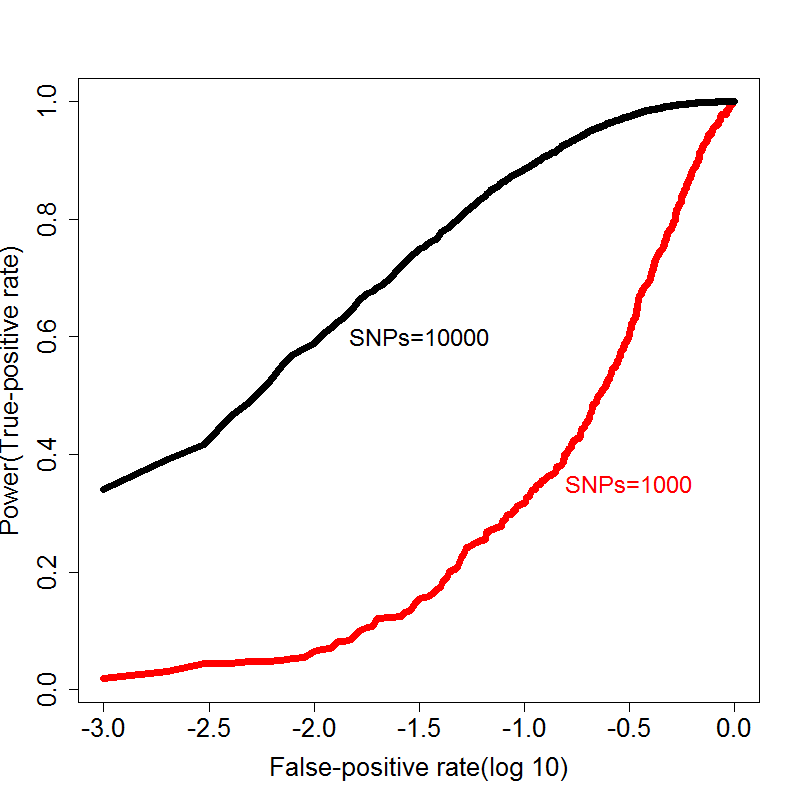
\includegraphics[width=0.4\textwidth]{snps.png}
		}%
		\subfigure[LR Test for Different Pretreatment]{%
			\label{fig:lr}
			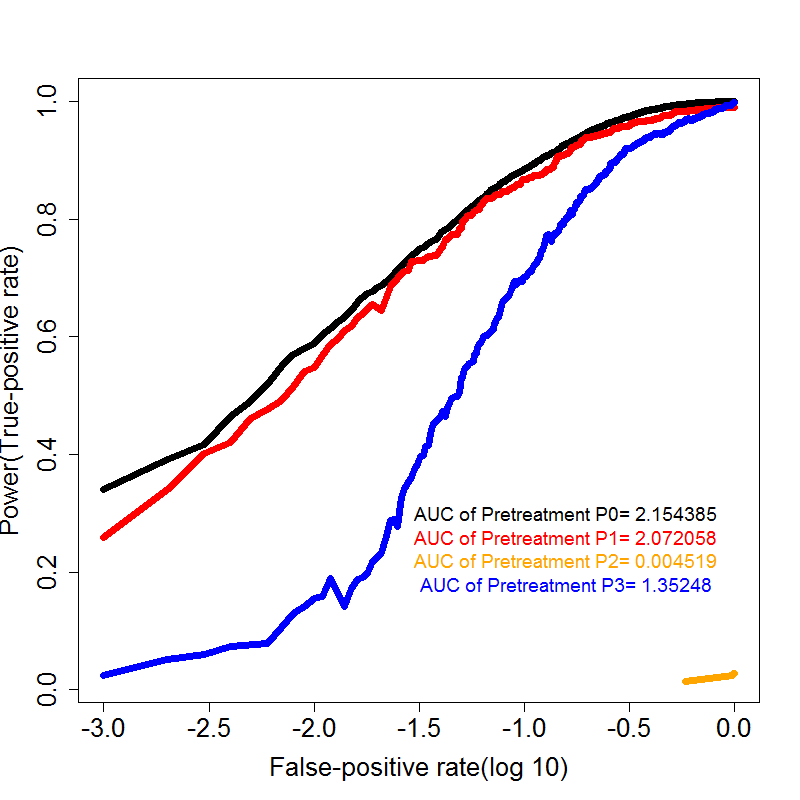
\includegraphics[width=0.4\textwidth]{lrtest.png}
		}
				%
				\subfigure[T1 test for Different Pretreatment]{%
					\label{fig:t1}
					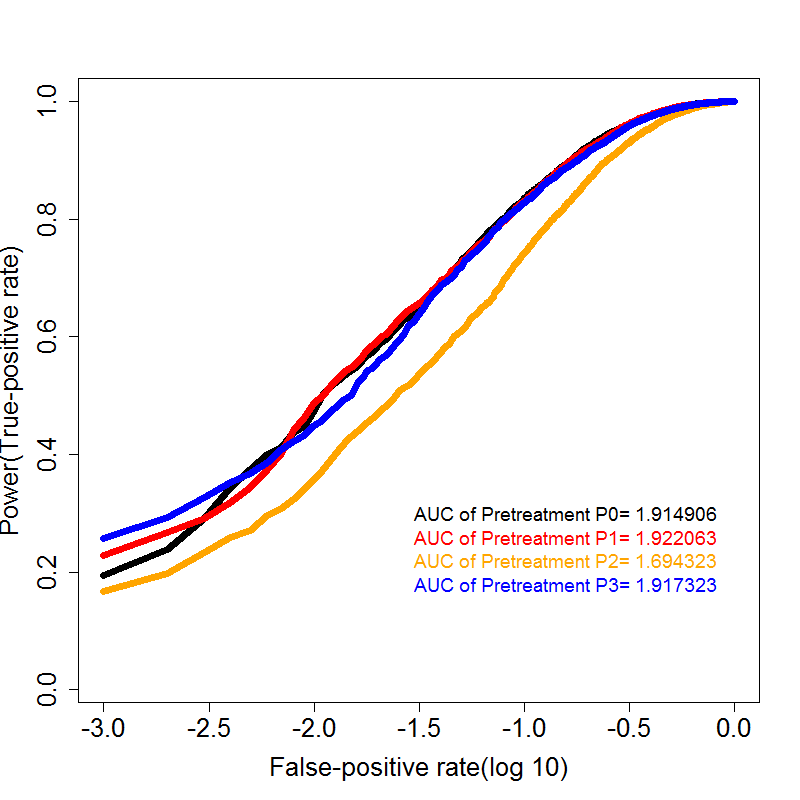
\includegraphics[width=0.4\textwidth]{t1test.png}
				}%
				\subfigure[T2 Test for Different Pretreatment]{%
					\label{fig:t2}
					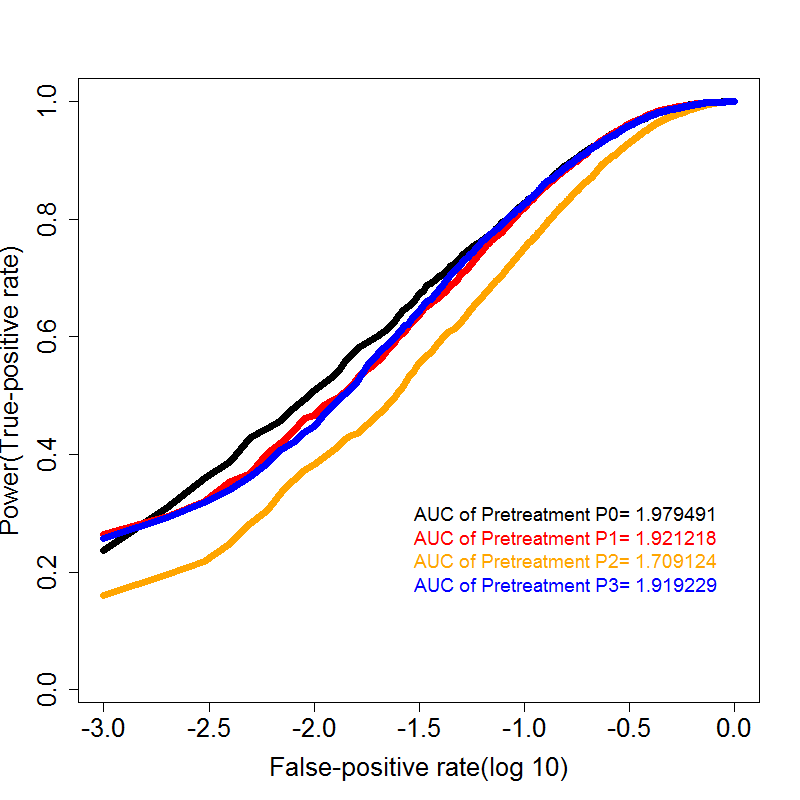
\includegraphics[width=0.4\textwidth]{t2test.png}
				}
	\end{center}
	\caption{%
Power of Different Tests. (a) The red and black solid line are corresponding ROC curve for LR test on SNP number= 1,000 and 10,000. (b-d) are different tests on different pretreatment, SNP number in thest tests are all 10,000. Black solid line is the ROC curve for pretreatment P0, red solid line is the ROC curve for pretreatment P1, orange solid line is the ROC curve for pretreatment P2 and blue solid line is the ROC for pretreatment P3. (b)LR test on different data pretreatment P0-P3 (c)T1 test on different data pretreatment P0-P3 (d)T2 test on different data pretreatment P0-P3
	}%
	\label{fig:subfigures}
\end{figure}

From Fig.~\ref{fig:lr} we can see LR test is very sensitive to pretreatment P2 and P3, which means that if we performs pretreatment P2 and P3, we have less privacy risk when releasing data in GWAS study. 

Compare Fig.~\ref{fig:t1} and Fig.~\ref{fig:t2} together with Fig.~\ref{fig:lr}, we can tell that T1 test and T2 test has less power than LR test on directly released data when predict whether certain individual is from pool or not. However, T1 test and T2 test is less sensitive to P2 and P3 pretreatment than LR test. Compare the AUC value of T1 and T2 test on each pretreatment, it is hard to tell if T1 is better than T2.
\section{Discussion}

In this project, we performs LR test, T1 test and T2 test on four different data pretreatments. According to our experiments, adding random Gaussian noise to SNPs frequency of pool(P3) and rounding to nearest multiple 0.1(P2) are two efficient method to defeat LR test. However, pretreatment P2 add too many noise into GWAS study, so we suggest perform Gaussian noise. 

In our experiment, we only test Gaussian noise with $\sigma=0.01$. The future work is to perform Gaussian noise with different $\sigma$. Meanwhile, As we discussed in 597I lecture, let $\epsilon\in(0,1)$ be arbitrary, For $c^2>2\mathrm{ln}(1.25/\delta)$, the Gaussian Mechanism with parameter $\sigma \ge c \Delta/\sigma$ is $(\epsilon,\delta)$- differentially private. Another future work is to perform differential private in GWAS.

Meanwhile, from our experiments we know T1 and T2 test is not sensitive to Gaussian noise, se T1 and T2 are good attack methods for released data with Gaussian noise.

\subsubsection*{Supplementary}
 All test dataset and experiment protocol for project reproduction can be achieved from this cite: (\url{https://www.dropbox.com/s/ahxn8eybafyx8i6/dataset.zip?dl=0}) $^*$ \cnote{* Test dataset can only be achieved before May 10th, 2015. For later achievement please contact the author.}
 
 We publish a tool called "privacy" that can perform all experiments in this project, source code and binary code can be achieved from \url{https://github.com/bbsunchen/privacy_gwas}.

\subsubsection*{Acknowledgements}

The author wish to express sicere thanks to Prof. Adam Smith for great lectures in 597I Spring2015 and patient discussions of this project. The author wish to express great thanks for readers' understanding of grammar errors in this report.
    
\bibliography{main}

\bibliographystyle{plain}

\end{document}
